\section{CIP Under Uncertainty}

This appendix describes a theoretical contribution that is separate from the rest of this thesis.  Covered interest parity is one of the basic concepts of international finance.  Its description --- that investing in a domestic or a foreign currency should give the same return --- is intuitive.  In a deterministic environment, it is a no-arbitrage condition.  The usual formula for CIP is:
\begin{equation} 
1 + r_{EUR} = S(1 + r_{USD})/F
 \end{equation}

However, in an environment with randomness, this formula does not have to hold by arbitrage.  We demonstrate this with a model that runs from $t=0$ to $t=2$, where the interest rates from $t=1$ to $t=2$ are random.  

\subsection{The Model}

My model is dervied from the Binomial Options Pricing Model\cite{Cox1979}.  However, instead of one stock price that can go up or down in the future, there are two interest rates (USD, EUR) that can go up or down.  

The initial state will be labeled $*$.  The state will transition to one of four second states $Uu$, $Ud$, $Du$, and $Dd$.  $U$ and $D$ indicate that the interest rate for USD has gone up or down, while $u$ and $d$ represent the same for EUR.  For simplicity, I assume all second states are equally probable.  

\begin{figure}[H]  % h = here
\textbf{\caption{\label{state_diagram} State Diagram}}
\centering
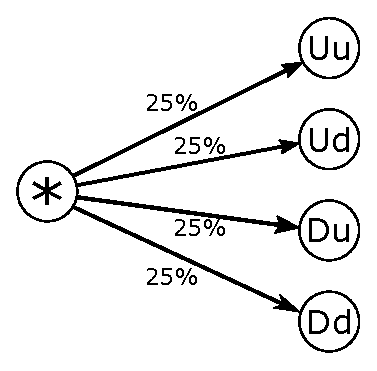
\includegraphics[height=2.1in]{images/state_diagram.eps}

\raggedright 
Note: {\small The initial state is labeled $*$.   There is an equal chance of going to any of four second states.  The second states are labeled with capital $U$ and $D$ if the USD interest rate goes up or down and with lowercase $u$ and $d$ if the EUR interest rate goes up or down.  In general, the initial state is concerned with the time period from $t=0$ to $t=1$ and the second states with $t=1$ to $t=2$.}
\newline Source: Bloomberg L.P. 
\end{figure}

For clarity, time is indexed separately from the state.  Time goes from $t=0$ to $t=2$.  In general, the initial state resolves values in the time period $t=0$ to $t=1$ and the second states resolve values in $t=1$ to $t=2$. 

Interest rates are calculated between two times.  $r_{c,t_1,t_2,s}$ is the interest rate for currency $c$ from time $t_1$ to time $t_2$ as calculated in state $s$.  The interests rates for USD and EUR from $t=0$ to $t=1$ are given and the same in all states.  In the initial state, those values are written $r_{USD,0,1,*}$ and $r_{EUR,0,1,*}$.  The interest rates for USD and EUR from $t=1$ to $t=2$ are given in the second states.  Thus, in state $Ud$, the value is $r_{USD,1,2,Ud}$.  

The interest rates for USD and EUR from $t=1$ to $t=2$ are \emph{not} given for the initial state, but these values could be estimated given traders behavior, the value in each of the second states, and the probability of transitioning to each second state.  This will be examined in the next section.

$S_{t,s}$ is the spot rate at time $t$ in state $s$.  The spot rate is given for time $t=2$ in all second states.  Thus, in state $Du$, the rate is written $S_{2,Du}$.  The spot rate is not given in $t=0$ nor $t=1$ for any state, but can be calcuated from other rates, as will be seen in the next section.


\subsection{Analysis}

Given the data known in the second states, the values for the spot price, forward price, and interest rates can be calculated for the initial state.  When we consider the values for the time span $t=0$ to $t=2$ in the initial state, only under certain conditions will those values obey the usual formula for CIP basis.  In general, they will not.

The value for the spot rate at time $t=1$ can calculated in each of the second states.  For any second state $s$, 
\begin{equation}
  S_{1,s} = \frac{1+r_{EUR,1,2,s}}{1 + r_{USD,1,2,s}} S_{2,s}
\end{equation}

\noindent This is just an application of the usual CIP formula, which can be applied here because the situation is completely deterministic.  

The value for the spot rate at time $t=1$ in the initial state is calculated from the values in each of the second states.  I assuming a risk-neutral measure, where a marketmaker buys and sells currency and treats profits and loses in any future state equally.  Thereby, the price is set at the expected value in each possible second state.
\begin{equation}
  S_{1,*} = \E[S_{1,s}]
\end{equation}

\noindent where $s$ is restricted to second states.

The spot rate's value at $t=0$ in the initial state is an application of the usual CIP formula, since the situation is deterministic inside the initial state.
\begin{align}
  S_{0,*} &= \frac{1+r_{EUR,0,1,*}}{1 + r_{USD,0,1,*}}\E[S_{1,s}]  \\
           &= \frac{1+r_{EUR,0,1,*}}{1 + r_{USD,0,1,*}}\E[\frac{1+r_{EUR,1,2,s}}{1 + r_{USD,1,2,s}} S_{2,s}]
\end{align}
\noindent where $s$ is restricted to second states.

$F_{t_1,t_2,s}$ is the price of a forward bought at $t_1$ with delivery date $t_2$, as calculated in state $s$.  We are only concerned with forwards that deliver at time $t=2$.  Inside a second state $s$, we know $F_{1,2,s} = S_{2,s}$ because we know the spot price at time $t=2$.  The forward price, in a deterministic environment, should be equal to it.

The price of a forward at $t=1$ in the initial state is set by a risk-neutral measure. 
\begin{equation}
  F_{1,2,*} = \E[F_{1,2,s}]
\end{equation}

\noindent where $s$ is restricted to second states.

The price of a forward at $t=0$ in the initial state is equal to the price at $t=1$ in the initial state, because it is a deterministic environment.  Thus:
\begin{align}
  F_{0,2,*} &= F_{1,2,*} \\
                &= \E[S_{2,s}]
\end{align}
\noindent for $s$ restricted to second states. 

Lastly, we need interest rates for the whole period from $t=0$ to $t=2$.  The interest rate for the second half, from $t=1$ to $t=2$, is given in each second state $s$ as $r_{c,1,2,s}$.  If interest profits follow a risk-neutral measure, the interest rate for the second half, as seen in the initial state, is the expected value of each possible state.  That is, $r_{c,1,2,*} = \E[r_{c,1,2,s}]$ for $s$ restricted to second states.  The interest rate for the whole $t=0$ to $t=2$ must then obey:
\begin{equation}
  (1 + r_{c,0,2,*})^2 = (1 + r_{c,0,1,*})(1 + \E[r_{c,1,2,s}])
\end{equation}

\noindent for each currency $c$ and second state $s$.

Now that we have the spot price, forward price and interest rates for the period $t=0$ to $t=2$ in the initial state, we can plug them into the usual CIP basis formula.  This yields:
\begin{equation}
  (1 + r_{EUR,0,2,*})^2 = S_{0,*}(1 + r_{USD,0,2,*})^2/F_{0,2,*}
\end{equation}

Substituting, we get:
\begin{multline}
  (1 + r_{EUR,0,1,*})(1 + \E[r_{EUR,1,2,s}]) =  \\ \frac{1+r_{EUR,0,1,*}}{1 + r_{USD,0,1,*}}\E[\frac{1+r_{EUR,1,2,s}}{1 + r_{USD,1,2,s}} S_{2,s}](1 + r_{USD,0,1,*})(1 + \E[r_{USD,1,2,s}])/\E[S_{2,s}]
%  \frac{1+r_{USD,0,1,s}}{1 + r_{EUR,0,1,s}}\E[\frac{1+r_{USD,1,2,s}}{1 + r_{EUR,1,2,s}} S_{2,s}] = \frac{(1 + r_{USD,0,1,*})(1 +\E[r_{USD,1,2,s}])}{(1 + r_{EUR,0,1,*})(1 +\E[r_{EUR,1,2,s}])} \E[S_{2,s}]
\end{multline}

Reducing, we get:
\begin{equation}
  \frac{(1 +\E[r_{USD,1,2,s}])}{(1 +\E[r_{EUR,1,2,s}])} \E[S_{2,s}] = \E[\frac{1+r_{USD,1,2,s}}{1 + r_{EUR,1,2,s}} S_{2,s}]
\end{equation}

As can be seen, the equation's terms are similar, but the expectation is in a different place on each side.  This means the CIP formula only holds under certain conditions.  We can identify those conditions by expanding the expectation and exposing the parameters $S_{2,s}$ for each of the second states: $Uu$, $Ud$, $Du$, and $Dd$.
\begin{equation}
  \frac{(1 +\E[r_{USD,1,2,s}])}{(1 +\E[r_{EUR,1,2,s}])} (.25S_{2,Uu}+.25S_{2,Ud}+.25S_{2,Du}+.25S_{2,Dd})  = 
.25\frac{1+r_{USD,1,2,Uu}}{1 + r_{EUR,1,2,Uu}}S_{2,Uu} + .25\frac{1+r_{USD,1,2,Ud}}{1 + r_{EUR,1,2,Ud}}S_{2,Ud} + .25\frac{1+r_{USD,1,2,Du}}{1 + r_{EUR,1,2,Du}}S_{2,Du} + .25\frac{1+r_{USD,1,2,Dd}}{1 + r_{EUR,1,2,Dd}}S_{2,Dd}
\end{equation}

We can rewrite to expose the factors to each parameter:
\begin{align}
  0 &= S_{2,Uu}( \frac{(1 +\E[r_{USD,1,2,s}])}{(1 +\E[r_{EUR,1,2,s}])} - \frac{1+r_{USD,1,2,Uu}}{1 + r_{EUR,1,2,Uu}}) \\
     &+ S_{2,Ud}(\frac{(1 +\E[r_{USD,1,2,s}])}{(1 +\E[r_{EUR,1,2,s}])} - \frac{1+r_{USD,1,2,Ud}}{1 + r_{EUR,1,2,Ud}}) \\
     &+ S_{2,Du}(\frac{(1 +\E[r_{USD,1,2,s}])}{(1 +\E[r_{EUR,1,2,s}])} - \frac{1+r_{USD,1,2,Du}}{1 + r_{EUR,1,2,Du}}) \\
     &+ S_{2,Dd}(\frac{(1 +\E[r_{USD,1,2,s}])}{(1 +\E[r_{EUR,1,2,s}])} - \frac{1+r_{USD,1,2,Dd}}{1 + r_{EUR,1,2,Dd}})
\end{align}

Since we know the parameters $S_{2,s}$ are non-zero, the only way for the equation to hold for all values of $S_{2,s}$ is if their factors are zero.  That gets us these 4 equations.  
\begin{align}
  \label{four-eqn} 
  \frac{(1 +\E[r_{USD,1,2,s}])}{(1 +\E[r_{EUR,1,2,s}])} &= frac{1+r_{USD,1,2,Uu}}{1 + r_{EUR,1,2,Uu}} \\
  \frac{(1 +\E[r_{USD,1,2,s}])}{(1 +\E[r_{EUR,1,2,s}])} &= frac{1+r_{USD,1,2,Ud}}{1 + r_{EUR,1,2,Ud}} \\
  \frac{(1 +\E[r_{USD,1,2,s}])}{(1 +\E[r_{EUR,1,2,s}])} &= frac{1+r_{USD,1,2,Du}}{1 + r_{EUR,1,2,Du}} \\
  \frac{(1 +\E[r_{USD,1,2,s}])}{(1 +\E[r_{EUR,1,2,s}])} &= frac{1+r_{USD,1,2,Dd}}{1 + r_{EUR,1,2,Dd}} 
\end{align}

The first two equations reduce to:
\begin{equation}
frac{1+r_{USD,1,2,Uu}}{1 + r_{EUR,1,2,Uu}} = frac{1+r_{USD,1,2,Ud}}{1 + r_{EUR,1,2,Ud}}
\end{equation}
\noindent Recall that the state names come from movements in the interest rates of each currency.  So, in both $Uu$ and $Ud$, the interest rate for USD is the same, because it has risen in both states.  So, $r_{USD,1,2,Uu} = r_{USD,1,2,Ud}$ and we get the first condition for the usual CIP formula being applicable to this random model:
\begin{equation}
  r_{EUR,1,2,Uu} = r_{EUR,1,2,Ud}
\end{equation}

\noindent That is, that there can be no difference in EUR interest rates between when it goes up or down.  That is, EUR's interest rates must be deterministic.

Combining the first and third equations in \eqref{four-eqn}, by a similar sequence of operations, produces:
\begin{equation}
  r_{USD,1,2,Uu} = r_{USD,1,2,Du}
\end{equation}

\noindent which means that USD interest rates must also be deterministic.

From this, I conclude that the usual formula for measuring CIP does not apply where there is randomness, or at least the type of randomness permitted by this model.  

\subsection{Application}

